\section{Comparison of {\asas} and {\harps} for period recovery}
\protect\label{section:asasfap}

It seemed appropriate to look in more detail at the {\asas} data which offers similar sampling to that from the {\harps}
data discussed in the preceding sections. Of particular importance is the False Alarm Probability of periods recovered
from the spectroscopic data as well as estimating the uncertainty level the calculated periods. None of the three Python
routines directly return an FAP and the the {\numrecs} routine always return an FAP of 1 if the periods were found at
all. Consequently a Monte Carlo method was devised and implemented to study this and at the same time help estimate the
uncertainty on the period obtained from the {\asas} results.

The main difference between the {\asas} and the {\harps} data is that the former have many more observations, 970,
although best results, as shown in Section \ref{section:asas}, were obtained if these were binned. If binned to 1 day,
there were 624 points, although the performance appeared best when binned to 18 minutes giving 924 data points. However
to compare ``like with like'' as much as possible, the 1-day binned data was taken.

So, starting from the {\asas} data, binned to 1 day and assuming for the purpose that the 82.6 day period obtained from
the full set as described in Section \ref{section:asas} is correct, various percentage-sized subsets of the data were
randomly selected, recalcaling the periods, noting whether a value close to the correct period was recovered as the
strongest peak, within the five strongest peaks, or not at all. If the period was recovered, the RMS error, assessed as
the difference from 82.6 days, was recorded. The sizes of the subsets were taken between 5\% and 95\% in steps of
5\%. For each percentage sized subset, the process was repeated 2,000 times. The results are illustrated in
Fig. \ref{fig:asasprop}.

In Fig. \ref{fig:asasprop} is shown four results. In all cases the X-axis displays the percentage sized subset of the
binned {\asas} data which was used. On the left Y-axis is shown the percentage of recovery (i.e. 100\% minus the FAP) of
the correct period. The blue line shows the percentage recovery of the correct period as the strongest peak with various
percentage sized subsets of the data and the green line shows the percentage recovery of the correct period as one of
the five strongest peaks, not necessarily as the strongest peak. If can be seen that former reaches 100\% recovery at
about 70\% and the latter at about 45\%.

On the right Y-axis is shown the RMS error in the period when it is correctly-recovered period. The purple line shows
the RMS error in the results corresponding to the case where the correct period is recovered as the strongest peak and
the red line the RMS error in the results corresponding to the case where the correct result is found in one of the top
five peaks. It is noticeable that this reaches less than 0.1 days in both cases, lending weight to the conclusion that
the uncertainty in the 82.6 peak found by {\asas} and {\hst} is of the order of 0.1 days.

Finally, marked in as the dotted vertical black lines are the number of points in the clipped and binned {\harps} data
for the Original Set of data to January 2014 (55 points) and the Full Set of data to March 2016 (89 points). It can be
seen the former intersects the blue line, representing the period being found at the strongest peak at just under 40\%
and the green line, where the period is found as one of the top five peaks, at just under 70\%. The equivalents for the
Full Set of data are just under 50\% and just over 80\% respectively.

These results can be compared with the results in Table \ref{table:perftable}, ignoring the last two columns. It can be
seen that in terms of finding the period in the top five peaks, Peak Ratios approach the level of recovery as the
{\asas} values for subsets with the same number of points, Skewness is perhaps half as good and Kurtosis a little
worse. Equivalent Widths are about the same as Kurtosis for the Full Set but are much worse for the Original
Set. However the RMS error is much worse for the Spectroscopic values, in the table the period was accepted if it fell
within 2\% of the values searched for, whereas the results from subsets of the {\asas} table had much better error
values. Also there were more points in the Specitroscopic values, Table \ref{table:perftable} is a condensation of the
results in Appendix \ref{chapter:pgramdetail} and therefore is rather better than reality.

\begin{figure}[!htbp]
\begin{center}
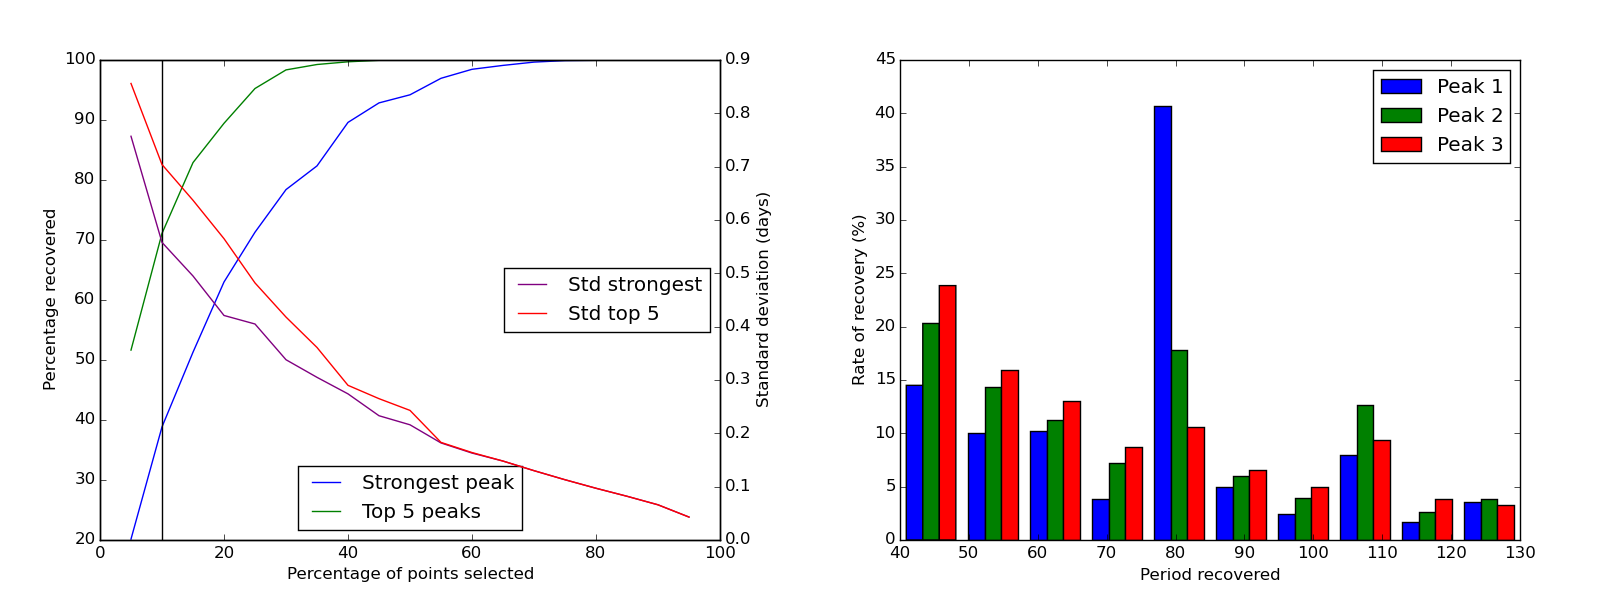
\includegraphics[scale=0.4]{Figures/prop.png} \\
\end{center}   
\caption{In this figure is illustrated the effects of randomly selecting a given proportion of the {\asas} data in terms
  of whether the same period of 82.6 days is recovered and the error in this result. The black vertical lines mark in
  the proportions of data in the 1 $\sigma$ clipping of the {\harps} date following by binning to 1 day of the Original
  Set and Full Set of data.}
\protect\label{fig:asasprop}
\end{figure}
